\chapter{Asking Palm Beach Billionaires How They Got So Rich}

This lecture unfolds as a search problem before it becomes a doctrine problem. We begin with a teaser reel of outsized claims and odd biographies, then the host places us in West Palm Beach, in a field said to contain more than sixty billionaires, and asks the governing question: by what mechanisms is wealth actually built here? What follows is not a blackboard derivation, but it does have a mathematical spine. The chapter therefore keeps close to the transcript and writes down only those formulas that sharpen the spoken mechanism: access under privacy, organic growth, staged scaling, delayed negotiation, institutional ascent, infrastructure demand, and leveraged ownership.

\section{Palm Beach as a Private Wealth Field}

The lecture opens by promising extremity. A strange answer about a rich brother-in-law, a billion-dollar business, a few hundred million in a year, and a \(\$54\) million case resolution are all flashed before us before the host pauses and tells us where we are. That ordering matters. First the spectacle, then the frame.

\paragraph{Anecdote.} West Palm Beach is introduced as one of the wealthiest cities not merely in Florida but in the world. The host then states the day's aim in the plainest possible terms: find very wealthy people and ask how they built their wealth and how someone else might become financially free in the present world.

\paragraph{Claim.} The numerical scene-setter is not decorative. It explains why the lecture immediately becomes a lesson in contact, skepticism, and persistence.
\begin{align}
N_{\mathrm{billionaires}} &> 60,\\
F_{\mathrm{host},1} &\approx 12.7\times 10^6,\\
F_{\mathrm{host},2} &\approx 5.4\times 10^6.
\end{align}
The first figure is the host's city-scale wealth claim; the latter two are host-stated audience sizes used as credibility in the field. They do not prove business truth. They explain why a stranger might stop for thirty seconds.

\paragraph{Mechanism.} We then watch refusals pile up. People are private. Some are wary, some annoyed, some simply moving. The lecture wants us to see this, because access is part of the content. The structure is not hidden:

\begin{figure}[h]
\centering
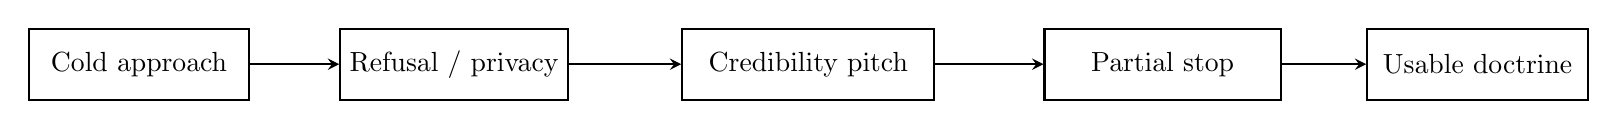
\begin{tikzpicture}[>=stealth, thick]
\node[draw, rectangle, minimum width=2.8cm, minimum height=0.9cm] (a) at (0,0) {Cold approach};
\node[draw, rectangle, minimum width=2.8cm, minimum height=0.9cm] (b) at (4,0) {Refusal / privacy};
\node[draw, rectangle, minimum width=3.2cm, minimum height=0.9cm] (c) at (8.5,0) {Credibility pitch};
\node[draw, rectangle, minimum width=3.0cm, minimum height=0.9cm] (d) at (13,0) {Partial stop};
\node[draw, rectangle, minimum width=2.8cm, minimum height=0.9cm] (e) at (17,0) {Usable doctrine};
\draw[->] (a) -- (b);
\draw[->] (b) -- (c);
\draw[->] (c) -- (d);
\draw[->] (d) -- (e);
\end{tikzpicture}
\caption{Transcript-derived access funnel. The lecture first solves the problem of contact, and only afterward extracts doctrine.}
\end{figure}

The host himself states the rule that converts embarrassment into method: \emph{no does not mean never; it means not yet}. That is the first serious sentence of the chapter.

\subsection{Question \& Answer}

\paragraph{Question.} Why does ``no'' not mean ``never'' in this setting?

\paragraph{Answer.} Because the lecture does not treat refusal as a final economic theorem. It treats refusal as the default friction of a privacy-heavy environment. The wealthy pedestrian is skeptical, but not always unreachable; what is required is repetition, brevity, and some socially legible proof that the request is real. This is why the host keeps returning to the same short access tools: audience size, prior interviews, and the promise of speed.

\section{From Rooftop Gravel to a Nationwide Vacuum-Truck Business}

Once the lecture earns a real stop, it gives us its strongest self-made operating arc. A man says that after college he got behind the wheel of a truck and sucked gravel off rooftops. He moves from this narrow manual specialty into industrial cleaning, then into power plants, refineries, and steel mills, and eventually into a nationwide vacuum-truck business and a nationwide liquid-storage-tank business.

\paragraph{Anecdote.} The oddity of the starting point must be preserved. The lecture wants us to feel how far the end state is from the beginning state. This is not a founder who begins with software, capital, or prestige. He begins with a dirty physical bottleneck and notices that the bottleneck scales.

\paragraph{Claim.} Two rules appear with almost no delay: he sold by knocking on doors cold, and he started with no outside money. When asked whether he borrowed or raised money, the answer is simply: nothing. That is the first clean financing claim of the lecture.

The first durable asset is priced explicitly:
\begin{align}
C_{\mathrm{truck},0} &= \$180{,}000,\\
C_{\mathrm{truck},\mathrm{now}} &\approx \$500{,}000\text{--}\$600{,}000.
\end{align}
The same interview later gives a durability statistic:
\begin{equation}
\frac{N_{\mathrm{closed\ offices}}}{N_{\mathrm{offices}}}=\frac{1}{40}.
\end{equation}
The point of the ratio is not elegance. It is to make survival visible.

\paragraph{Mechanism.} The speaker's growth model is the simplest one in the lecture: profits are put back into the business. A careful shorthand is
\begin{equation}
K_{t+1}=K_t+\pi_t^{\mathrm{retained}},
\end{equation}
where \(K_t\) denotes productive operating capital and \(\pi_t^{\mathrm{retained}}\) retained profit. This is an editorial compression, not a quoted formula, but it captures exactly what the speaker says the firm did.

The same speaker insists that scale should not be imagined as a jump:
\begin{equation}
0 \not\to 100,\qquad 0 \to 5 \to 10 \to 15.
\end{equation}
We should keep the staircase in precisely this spirit: not a law of nature, but a lecture-grade image of staged growth.

\begin{figure}[h]
\centering
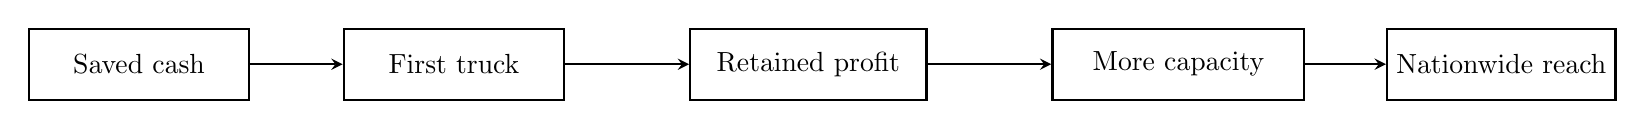
\begin{tikzpicture}[>=stealth, thick]
\node[draw, rectangle, minimum width=2.8cm, minimum height=0.9cm] (a) at (0,0) {Saved cash};
\node[draw, rectangle, minimum width=2.8cm, minimum height=0.9cm] (b) at (4,0) {First truck};
\node[draw, rectangle, minimum width=3.0cm, minimum height=0.9cm] (c) at (8.5,0) {Retained profit};
\node[draw, rectangle, minimum width=3.2cm, minimum height=0.9cm] (d) at (13.2,0) {More capacity};
\node[draw, rectangle, minimum width=2.8cm, minimum height=0.9cm] (e) at (17.3,0) {Nationwide reach};
\draw[->] (a) -- (b);
\draw[->] (b) -- (c);
\draw[->] (c) -- (d);
\draw[->] (d) -- (e);
\end{tikzpicture}
\caption{Transcript-derived bootstrap loop from first asset to broader operating footprint.}
\end{figure}

One more point from this same stretch should not be lost. Asked about vertical integration, the speaker does not answer with supply-chain theory; he answers that the hardest part of business is people, meaning management. That is entirely in character with the lecture. The binding constraint is seldom a diagram; it is often a human system.

\subsection{Question \& Answer}

\paragraph{Question.} How does scale emerge from zero when no outside capital is raised?

\paragraph{Answer.} The lecture's answer is recursive rather than heroic.

\begin{enumerate}
\item Save enough cash to acquire the first productive asset.
\item Use that asset to perform a specialized task that customers already pay for.
\item Retain profit instead of distributing it.
\item Reinvest retained profit in more equipment, more geography, or more service lines.
\item Repeat until the business footprint is larger than the founding asset.
\end{enumerate}

This is why the speaker immediately adds two ethical-looking but actually economic conditions: think long term, and do work you can love for decades. If the financing loop is slow, then patience and internal motivation are not slogans. They are feasibility conditions.

\section{Mortgage Timing, Plaintiff Law, and the Discoverability Pivot}

The lecture now widens its field. One speaker says he made his first million at \(25\) in mortgage banking in San Francisco. The explanation is blunt and concrete: real estate in California, and especially San Francisco, was booming. Wealth here is tied to standing at the right intersection of geography and timing.

The next speaker, a personal-injury and mass-tort lawyer, turns the chapter in a different direction. He says the legal business made him the most money and gives the lecture its clearest money anchors from the legal world:
\begin{align}
S_{\mathrm{case}} &= \$54\,\mathrm{M},\\
S_0 &= \$30\,\mathrm{M},\\
S_1 &> \$50\,\mathrm{M}.
\end{align}
These are case-resolution figures. The notes must keep them in that form and resist silently converting them into fee income or annual firm revenue.

\paragraph{Claim.} The lawyer's account is really about discoverability. First he says that he became an expert at SEO and advertised on the web before it was popular; that is how the firm launched. Then, when pressed for present advice, he reverses the emphasis and says not to pursue SEO now, but to market on social media. The lecture thus keeps the underlying rule fixed while allowing the surface tactic to change: the best operator in the room still loses if nobody knows where to find him.

\paragraph{Mechanism.} The same interview contributes a second mechanism: stronger rooms preserve wealth. The speaker says the goal is to be the dumbest person in the room. In this lecture that line is not self-help rhetoric; it is an allocation rule. Capital is stabilized when expertise around it exceeds the owner's expertise.

\subsection{Question \& Answer}

\paragraph{Question.} Why leave \(\$30\,\mathrm{M}\) on the table?

\paragraph{Answer.} Because the lecture treats time as part of the bargaining instrument. The simplest worked comparison is
\begin{align}
S_1-S_0 &> \$20\,\mathrm{M},\\
S_1 &> S_0.
\end{align}
The speaker's formulation is memorable: do not be prepared to do the deal at the table; be prepared to do the deal outside the room. In the specific case he gives, delay dominates immediate closure.

\begin{enumerate}
\item A very large present offer appears.
\item The negotiator refuses to identify largeness with finality.
\item The case remains live.
\item Bargaining pressure continues to evolve outside the room.
\item The later settlement exceeds the earlier one.
\end{enumerate}

The host immediately recaps this answer for the audience, and that recap is worth retaining. The interview is not merely about legal skill; it is about the long game defeating instant gratification.

\section{The Corporate Ladder as a Wealth Path}

At this point the lecture changes archetype. Up to now we have mostly been watching founders and owner-operators. The next major speaker is different: an unnamed public-company CEO who says he worked for one business-services company his entire career and eventually became its chief executive.

\paragraph{Anecdote.} The shift in texture matters. The lecture is no longer telling us how to build a company out of nothing. It is telling us that large wealth and authority can also emerge inside an existing institution, provided the institution is large enough and its culture is porous enough.

\paragraph{Claim.} The scale markers are not small:
\begin{align}
N_{\mathrm{employees}} &= 42{,}000,\\
T_{\mathrm{CEO}} &= 18\ \mathrm{years}.
\end{align}
The company is also described as doing multi-billions of dollars in annual revenue and maintaining high-single-digit growth over fifty years. This is the lecture's cleanest employee-to-operator case.

\subsection{Question \& Answer}

\paragraph{Question.} How does someone actually work up to CEO inside a giant company?

\paragraph{Answer.} The speaker gives an answer that is procedural, almost algorithmic.

\begin{enumerate}
\item Finish the assigned work for the day.
\item Ask the boss what else needs to be done.
\item Take on tasks that would otherwise remain with the boss.
\item Learn the next layer of the organization by doing those tasks.
\item Become legible as the boss's right-hand person.
\item Be the obvious choice when a larger opportunity appears.
\item Perform well at the higher level and repeat.
\end{enumerate}

The lecture likes this answer because it makes the climb imaginable. What had seemed unreasonable a moment earlier is converted into a repeatable loop of delegated work, trust, and performance.

\paragraph{Mechanism.} The speaker later adds the two human sources from which he learned most: his father and his predecessor as CEO. This detail matters because it prevents the corporate ladder from being read as a purely impersonal machine. Institutional ascent still depends on transmitted judgment.

\section{Pressure, Responsibility, and the Frog-in-the-Kettle Rule}

Once the corporate climb has been described, the host asks the next natural question: what happens to the human being who has \(42{,}000\) employees, investors, customers, and public expectations pressing against him? The lecture does not evade the scale of this burden.

\paragraph{Mechanism.} The answer is not that pressure disappears, but that one becomes more used to carrying it. A cautious transcript-led schematic is
\begin{equation}
P_{t+1}>P_t,\qquad \Theta_{t+1}>\Theta_t,
\end{equation}
where \(P_t\) is role pressure and \(\Theta_t\) tolerance to pressure. This is not a quantitative law; it is the cleanest mathematical restatement of the speaker's frog-in-the-kettle analogy.

\begin{figure}[h]
\centering
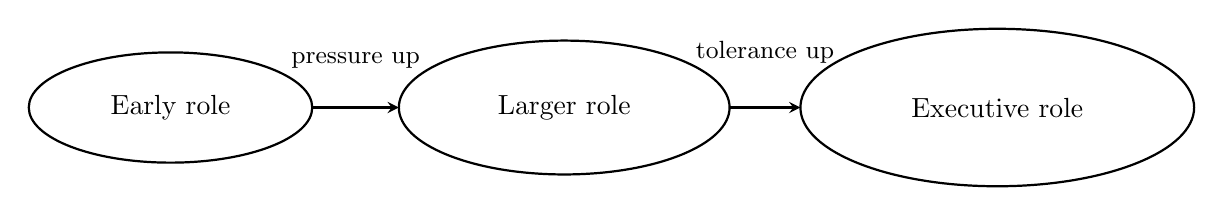
\begin{tikzpicture}[>=stealth, thick]
\draw[draw] (0,0) ellipse (1.8 and 0.7);
\node at (0,0) {Early role};
\draw[draw] (5,0) ellipse (2.1 and 0.85);
\node at (5,0) {Larger role};
\draw[draw] (10.5,0) ellipse (2.5 and 1.0);
\node at (10.5,0) {Executive role};
\draw[->] (1.8,0) -- (2.9,0);
\draw[->] (7.1,0) -- (8.0,0);
\node at (2.35,0.6) {\small pressure up};
\node at (7.55,0.7) {\small tolerance up};
\end{tikzpicture}
\caption{Transcript-derived pressure-acclimation schematic: advancement increases difficulty, but it also increases one's capacity to absorb it.}
\end{figure}

\begin{enumerate}
\item Responsibility rises as one moves upward.
\item Harder problems therefore appear.
\item Repeated exposure weakens the tendency to overreact.
\item One does not escape hard problems; one becomes more able to metabolize them.
\end{enumerate}

\paragraph{Transition.} The corporate segment ends with an unfinished question about the lowest point in a career, and then with a darker line: business contains more problems than upside moments. That is the right place for the lecture to pause. The tone has shifted from ascent to burden, and only then does the host briefly insert the narrower point about online presence and websites before returning to another wealthy operator.

\section{AI Infrastructure, Diversification, and Relationship Selling}

After the brief website interlude, the lecture re-enters through industrial infrastructure. One interviewee says he made his first million at \(42\), is now running a business on the order of a billion in scale, had roughly \(\$500\,\mathrm{M}\) of order intake in one year, and once closed a single customer order of roughly \(\$250\,\mathrm{M}\).

\paragraph{Claim.} The important conceptual move is that AI enters here not as software magic but as demand for physical capacity. The speaker says that an AI search is roughly ten times a Google search:
\begin{equation}
\frac{L_{\mathrm{AI\ search}}}{L_{\mathrm{Google\ search}}}\approx 10.
\end{equation}
We should keep this as a speaker-attributed heuristic. Its value in the lecture is structural, not experimental.

\subsection{Question \& Answer}

\paragraph{Question.} How does AI create money for a company that is not itself an AI company?

\paragraph{Answer.} The lecture's answer is a causal chain from compute intensity to power demand to equipment demand.
\begin{equation}
L_{\mathrm{AI\ load}}\uparrow \;\Rightarrow\; P_{\mathrm{data\ center}}\uparrow \;\Rightarrow\; Q_{\mathrm{generator}}\uparrow.
\end{equation}

\begin{enumerate}
\item AI-style queries require heavier computation than ordinary search.
\item Heavier computation increases data-center load.
\item Larger load raises both standby-power and baseload-power requirements.
\item Businesses that supply generators and related equipment therefore gain demand even if they do not build AI products.
\end{enumerate}

\paragraph{Mechanism.} The rest of this interview is not just about demand but about how demand is monetized. The speaker says he has both geographical diversity and sector diversity; that is one stabilizer. The other is relationship design. A \(\$250\) million order is not presented as a mere specification sheet. It is presented as a consequence of trust, reassurance, and adaptation to the customer's own world. Bankers, oil-and-gas operators, and large-market executives are not approached in the same social register.

The most concrete management image from this section is the glass office door. The speaker identifies communication and transparency as his superpower: not because transparency is morally beautiful, but because it lowers the fear and rumor that grow when decisions occur behind opaque walls.

\section{Private Equity, Leverage, and the Velocity of Cash}

The last major interview closes the chapter by making the capital structure explicit. The speaker has been in several businesses and is now in private equity. Asked whether one should start or buy a business in today's world, he says: buy. The reason is not mystical. A business with a track record is legible to a bank in a way that a pure start-up often is not.

\paragraph{Claim.} The lecture's private-equity model is given in simple verbal form: buy a company, borrow against the assets of that company, and pay the borrowing down through the cash flow of the business. A cautious symbolic version is
\begin{align}
D_t &\le A_t,\\
CF_t &\ge DS_t.
\end{align}
Here \(A_t\) is the asset base, \(D_t\) the debt raised against it, \(CF_t\) the cash flow, and \(DS_t\) the debt-service requirement. The speaker does not write these symbols, but the structure is unmistakable.

\begin{figure}[h]
\centering
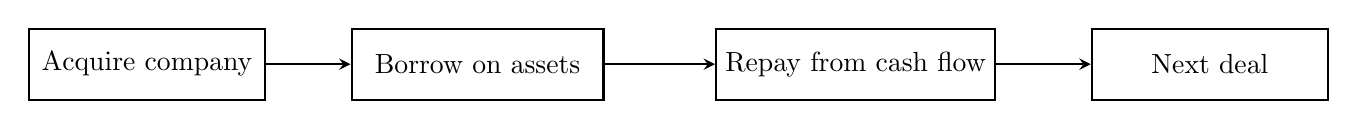
\begin{tikzpicture}[>=stealth, thick]
\node[draw, rectangle, minimum width=3.0cm, minimum height=0.9cm] (a) at (0,0) {Acquire company};
\node[draw, rectangle, minimum width=3.2cm, minimum height=0.9cm] (b) at (4.2,0) {Borrow on assets};
\node[draw, rectangle, minimum width=3.4cm, minimum height=0.9cm] (c) at (9.0,0) {Repay from cash flow};
\node[draw, rectangle, minimum width=3.0cm, minimum height=0.9cm] (d) at (13.5,0) {Next deal};
\draw[->] (a) -- (b);
\draw[->] (b) -- (c);
\draw[->] (c) -- (d);
\end{tikzpicture}
\caption{Transcript-derived private-equity loop: acquisition, asset-backed borrowing, cash-flow repayment, and renewed acquisition capacity.}
\end{figure}

\subsection{Question \& Answer}

\paragraph{Question.} What makes private equity work, and why is buying often easier than starting?

\paragraph{Answer.} Because, in the lecture's own terms, buying begins with a business that already has a financial history, an asset base, and some bank legibility.

\begin{enumerate}
\item The target business has assets that can support lending.
\item The target business has cash flow that can service lending.
\item The bank therefore lends against an operating reality rather than only against a founder's promise.
\item Debt is repaid from the business.
\item Reputation with banks accumulates across deals.
\end{enumerate}

This is also where the lecture most explicitly ties wealth to risk. The speaker says that the most successful people he knows are willing to take risk, and gives his own second deal as the example: he leveraged his house and everything he had. The lecture does not celebrate recklessness, but it plainly refuses safety as the usual path to great wealth.

\paragraph{Mechanism.} The last mathematical idea is the distinction between margin and velocity of cash. The speaker invokes Walmart: low margin, fast turns, large aggregate profit. A careful summary is
\begin{equation}
\Pi_{\mathrm{period}} \propto m\cdot v,
\end{equation}
where \(m\) denotes margin per turn and \(v\) the number of cash turns in the period. The point is not the proportionality sign itself. The point is to break the bad habit of evaluating a business by margin alone.

The interview closes with a directional thesis rather than a theorem: U.S.\ manufacturing, onshoring, and the continued purchase of domestic manufacturing companies. It is also the place where the lecture states its bluntest ownership claim. One may become wealthy as the CEO of a company, but if one wants to get rich, the interviewee says, one should own the business.

\section{Summary}

The lecture begins with a hunt for access and ends with a compact theory of how wealth is built across several different forms of economic life. We see a manual niche become a capital loop; a professional service become a discoverability problem; a legal negotiation become an exercise in delayed payoff; a corporate career become a ladder of delegated work and rising tolerance; AI become power demand; and private equity become a machine for turning assets and cash flow into renewed acquisition capacity. What gives the lecture its coherence is not that every route is the same, but that each route eventually exposes the same backbone: patience, ownership, trust, reinvestment, and the willingness to let time, rather than appetite, govern the large decision.